\chapter{Meta-phasing: methods for generating consensus phase from multiple algorithms}
\label{chpt:metaphase}

In chapter \ref{chpt:phasingEval} we evaluated the distribution of errors generated by three phasing algorithms. One way in which we could aggregate the results for each sample across the three methods would be to take a consensus voting approach, in which the phase at each heterozygous position would be that in which at least two methods were in agreement. Similar to \citep{AlBkhetan2020}, we describe the consensus vote approach in \ref{alg:cp}:

\begin{algorithm}
\caption{Consensus Phase Algorithm}\label{alg:cp}
\begin{algorithmic}
\State \textbf{Input}:  $\{h_1, h_2, h_3\} - \textrm{phasing estimates, } h_j \in \{0,1\}^p$
\State \textbf{Output: } \textit{cons} $\in \{0,1\}^p$
\For{$i = 0, \ldots, p$}
\State $cons[i] \gets majority\_vote(h_1[i], h_2[i], h_3[i])$
\For{$j = 1, 2, 3$}
\If{$h_j[i] \ne cons[i]$}
\State $h_j[i:p] = complement(h_j[i:p])$
\EndIf
\EndFor
\EndFor
\end{algorithmic}
\end{algorithm}

\begin{figure}
    \centering
    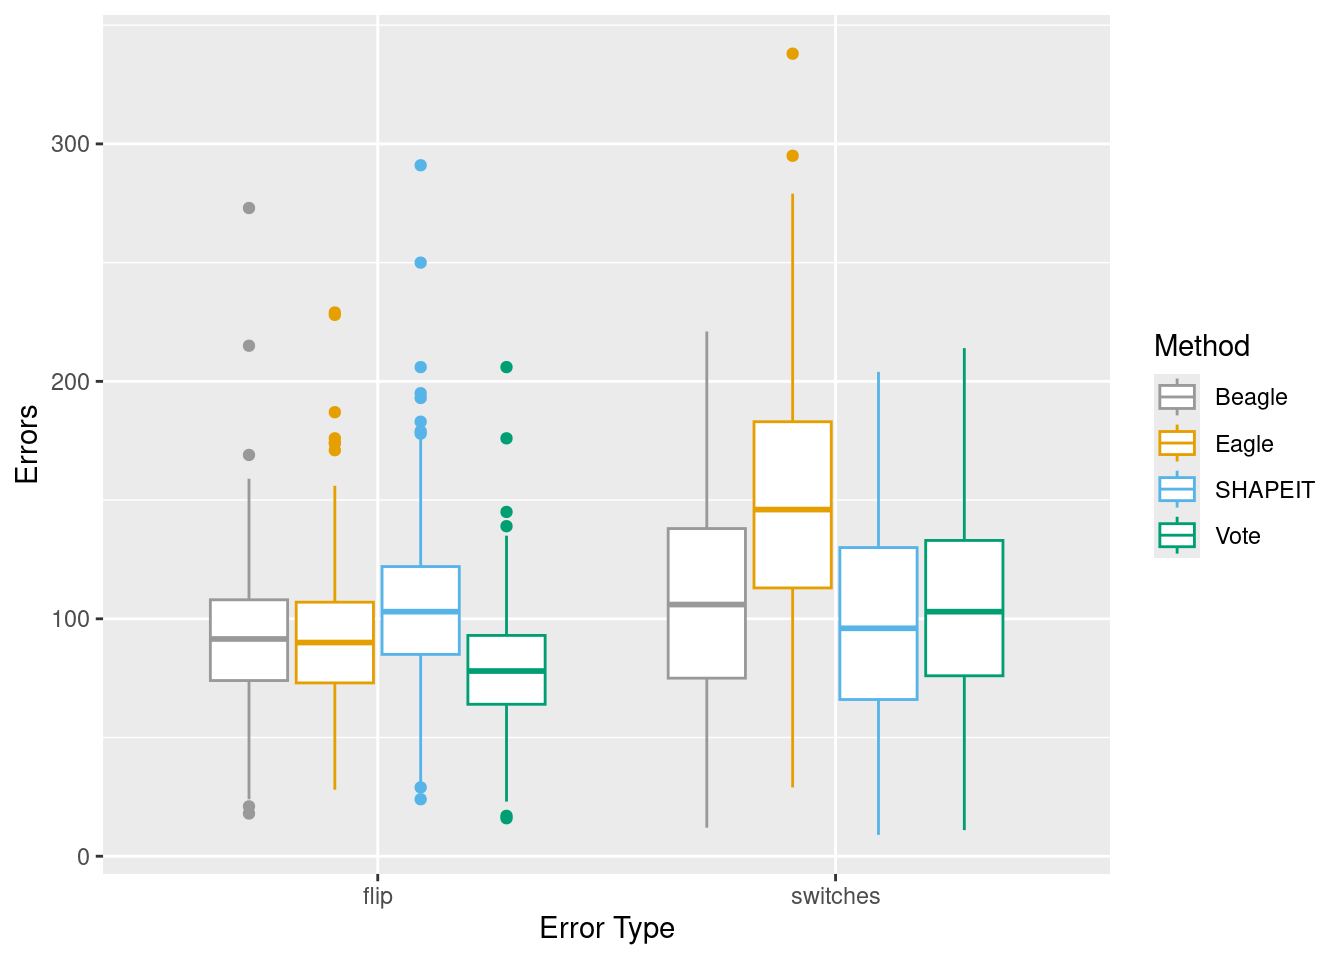
\includegraphics[scale=0.90]{chapters/figures/vote_results.png}
    \caption{Switch and flip error rate distributions over 1000 synthetic diploids by phasing method. While we generally see lower flip rates from the consensus vote approach, we don't see much of an improvement for switch error rates.}
    \label{fig:vote}
\end{figure}

When we apply the consensus vote approach to our X chromosome synthetic diploids, we see a modest improvement in flip error rates, but we don't see an improvement in switch error rates (figure \ref{fig:vote}). This is unsurprising given the extent to which we observe errors being shared across methods for each individual. In this chapter we aim to improve on the consensus vote approach by exploring alternative ways to combine results from multiple phasing algorithms. 

In the first phase of the project, we will explore error models individual phasing results. Given the sequential nature of chromosomes and how their phase can be represented as a binary vector, we will first explore models of the form seen in equation \ref{eq:phase_error}:

\begin{equation}
\label{eq:phase_error}
    e_{i,j} = \Pr(\textrm{error at position } i \textrm{, sample } j) = f(i, j) 
\end{equation}

where $f$ represents a generic class of functions that returns a probability of an error occurring at a position given some yet to be defined set of features. This set of features likely will include information on the genomic context at the position, such as average recombination rates in regions around that position in the chromosome. Additionally, we will consider ways to incorporate the sequential nature of chromosomes in these models, sharing information across neighboring heterozygous positions which might also be informative to the probability of a switch occuring at a position.

For the task of meta-phasing, we will first consider hidden markov models (HMMs), were we observe the inferred phase from multiple algorithms at each heterozygous position. We can represent these as a single binary vector where we track where each algorithm decides to place the non-reference allele realtive to the chromosome with the non-reference allele at the first heterozygous position 
(i.e., $h \in \{0,1\}^p$, $h[1] = 1$).
For the unobserved latent variable at each position, we have several options to consider, the most obvious of which is the true underlying phase at the position. In this model, the transition probabilities would then be the probability of observing either the reference or alternative allele on the true phased chromosome at the next position given the phase at the current position, and the emission probabilities would reflect whether or not each algorithm was inferring the correct phase given the true underlying state.

Another option for the hidden latent state in an HMM is to attach an indicator for each algorithm representing whether or not at the position the algorithm is placing reference and alternative alleles onto the right chromosome (equivalently, we can consider only the chromosome with the alterative allele at the first heterozygous position, in which case the indicator reflect whether the algorithm is placing the correct variant on this one chromosome). Transition probabilities from above would then be augmented with switch rates for each algorithm, while emission probabilities would either be 0 or 1, depending on the true phase at the position and the error status of the method.